\chapter{الترموديناميك الإحصائي: دوال التجزئة}\label{ch:b3:partition-functions}

يحمل قبر لودفيغ بولتزمان في فيينا سطرًا واحدًا، $S = k\log W$: فإنتروبيا
النظام تعدّ الطرائق التي تستطيع بها جزيئاته أن تتقاسم طاقته.
والترموديناميك، كما بناه مجلدا السنة الأولى والسنة الثانية، لا يحتاج أبدًا إلى
الجزيئات: فهو يربط الحرارات والإنتروبيات وثوابت التوازن المقيسة بعضها
ببعض. أما الترموديناميك الإحصائي فيحسبها انطلاقًا من الجزيئات
نفسها. وموضوعه المركزي مجموع واحد على مستويات طاقة جزيء
واحد، هو دالة التجزئة؛ والمستويات تأتي من المطيافية، 
والإنتروبيا القياسية للنيتروجين المحسوبة من طيفه توافق
القيمة الجدولية حتى جزء من مئة من الجول لكل كلفن ولكل مول. يبني هذا الفصل
دالة التجزئة، ويقسمها إلى أجزائها الانسحابية والدورانية
والاهتزازية والإلكترونية، ويحوّلها إلى طاقة داخلية وإنتروبيا
وطاقة جيبس؛ ويطبّقها \cref{ch:b3:statistical-thermo-applied} على السعات
الحرارية وثوابت التوازن.

\begin{recall}
عرّف مجلد السنة الثانية الإنتروبيا المولية القياسية وطاقة جيبس 
والجهد الكيميائي، وجدول الإنتروبيات المستخرجة من سعات حرارية
مقيسة حتى درجات حرارة منخفضة. وأعطى \cref{ch:b3:quantum-model-systems}
مستويات طاقة \omterm{def:b3:quantum-model-systems:box}{جسيم في صندوق}، \omterm{def:b3:quantum-model-systems:oscillator}{والهزاز التوافقي}، 
\omterm{def:b3:quantum-model-systems:rotor}{والدوّار الصلب}، $E_J = hcBJ(J+1)$ \omterm{def:b3:quantum-model-systems:degenerate}{بدرجة انحلال} $2J + 1$؛
وقاس \cref{ch:b3:rovibrational-spectroscopy} $B$ و$\tilde\nu$ للجزيئات
الثنائية الذرة ووجد أن سبينات النوى في جزيء متجانس النواتين مثل \ce{N2}
تجعل المستويات الدورانية المتناوبة غير متساوية.
\end{recall}

\section{الحالات المجهرية وتوزيع بولتزمان}

لنأخذ $N$ جزيئًا متطابقًا مستقلًا يمكنها أن تشغل مستويات طاقتها
$\varepsilon_0 = 0 < \varepsilon_1 < \varepsilon_2 < \dots$، وطاقتها الكلية $E$. وذكر عدد
الجزيئات في كل مستوى، $\{n_0, n_1, \dots\}$، يصف توزيعًا؛ أما
ذكر أي جزيء في أي مستوى فيصف أكثر من ذلك بكثير.

\begin{definition}[الحالة المجهرية، الوزن الإحصائي]\label{def:b3:partition-functions:microstate}
\emph{الحالة المجهرية}\index{حالة مجهرية} لنظام من الجزيئات تحديد
كامل لحالة كل جزيء. و\emph{الوزن
الإحصائي}\index{وزن إحصائي} $W$ لتوزيع $\{n_i\}$ لعدد $N$ من الجزيئات على
مستويات غير منحلة هو عدد الحالات المجهرية التي تحققه:
\[
  W = \frac{N!}{n_0!\,n_1!\,n_2!\cdots}.
\]
\end{definition}

\begin{example}[ثلاثة كمّات بين ثلاثة هزازات]\label{ex:b3:partition-functions:three-quanta}
تتقاسم ثلاثة هزازات ثلاثة كمّات من الطاقة. فالتوزيع «هزاز
واحد يحمل الكمّات الثلاثة» يتحقق بعدد $3!/(1!\,2!) = 3$ طرائق، و«واحد
يحمل اثنين، وآخر واحدًا» بعدد $3! = 6$ طرائق، و«كل منها يحمل واحدًا» بطريقة واحدة:
فالمجموع عشر \omterm{def:b3:partition-functions:microstate}{حالات مجهرية}، والتوزيع الأكثر انتظامًا الذي ما زال ينشر
الطاقة على عدة مستويات هو الأكثر احتمالًا. ومع $10^{23}$ جزيئًا تصبح
الأوزان حادة الذروة إلى حد أن توزيعًا واحدًا، والتوزيعات التي لا تختلف
عنه إلا بمقدار مهمل، تحمل عمليًا كل \omterm{def:b3:partition-functions:microstate}{الحالات المجهرية}.
\end{example}

\begin{remark}
مسلّمة الترموديناميك الإحصائي أن كل \omterm{def:b3:partition-functions:microstate}{الحالات المجهرية} لنظام
معزول ذي طاقة معينة متساوية الاحتمال. فيوجد النظام عندئذ،
بأرجحية ساحقة، في التوزيع ذي الوزن الأكبر: وإيجاده هو
مهمة هذا القسم.
\end{remark}

من أجل الأعداد الكبيرة، يعطي تقريب ستيرلنغ $\ln x! \approx x\ln x - x$
\[
  \ln W = N\ln N - \sum_i n_i\ln n_i .
\]

\begin{definition}[توزيع بولتزمان، الإشغال]\label{def:b3:partition-functions:boltzmann}
\emph{إشغال}\index{إشغال} مستوى ما $n_i/N$ هو نسبة
الجزيئات التي تشغله. و\emph{توزيع بولتزمان}\index{توزيع بولتزمان}
هو التوزيع ذو الوزن الأكبر لجزيئات مستقلة في
توازن حراري عند درجة الحرارة $T$، وتعطيه المبرهنة أدناه.
\end{definition}

\begin{theorem}[توزيع بولتزمان]\label{thm:b3:partition-functions:boltzmann}
من أجل جزيئات مستقلة في توازن عند درجة الحرارة $T$، يكون \omterm{def:b3:partition-functions:boltzmann}{إشغال}
مستوى طاقته $\varepsilon_i$ \omterm{def:b3:quantum-model-systems:degenerate}{ودرجة انحلاله} $g_i$
\[
  \frac{n_i}{N} = \frac{g_i\eu^{-\varepsilon_i/kT}}{q},
  \qquad q = \sum_i g_i\eu^{-\varepsilon_i/kT},
\]
حيث $k$ ثابت بولتزمان. ونسبة إشغالي مستويين هي
$\frac{n_j}{n_i} = \frac{g_j}{g_i}\eu^{-(\varepsilon_j - \varepsilon_i)/kT}$.
\end{theorem}

\begin{proof}[برهان جزئي]
لنأخذ أولًا مستويات غير منحلة. لنجعل $\ln W$ أكبر ما يمكن تحت القيدين
$\sum_in_i = N$ و$\sum_in_i\varepsilon_i = E$ بمضروبي لاغرانج $\alpha$ و$\beta$:
من أجل كل $i$،
\[
  \frac{\partial}{\partial n_i}\Bigl(\ln W + \alpha\sum_jn_j - \beta\sum_jn_j\varepsilon_j\Bigr)
  = -\ln n_i - 1 + \alpha - \beta\varepsilon_i = 0,
\]
ومنه $n_i = \eu^{\alpha - 1}\eu^{-\beta\varepsilon_i}$، ويثبّت القيد الأول $\eu^{\alpha - 1}
= N/\sum_j\eu^{-\beta\varepsilon_j}$. والمستوى ذو \omterm{def:b3:quantum-model-systems:degenerate}{درجة الانحلال} $g_i$ هو $g_i$ حالة متمايزة لها
الطاقة نفسها، كل منها مشغولة كما سبق: فيُضرب إشغاله في
$g_i$. ويُعيَّن المضروب $\beta$ بحالة واحدة معروفة: فمن أجل
الحركة الانسحابية لغاز مثالي (\cref{prop:b3:partition-functions:q-trans}
أدناه) يعطي التوزيع طاقة $\frac32N/\beta$، وطاقة الغاز المثالي
$\frac32NkT$؛ ومنه $\beta = 1/kT$. أما أن $\beta$ المقدار نفسه لكل
نوع من الحركة، وأنه درجة الحرارة الترموديناميكية، فنقبله
هنا دون برهان: فالنظامان المتلامسان حراريًا يتقاسمان $\beta$ نفسه، وهذه هي الخاصية
المعرِّفة لدرجة الحرارة.
\end{proof}

\begin{definition}[دالة التجزئة الجزيئية]\label{def:b3:partition-functions:partition-function}
\emph{دالة التجزئة الجزيئية}\index{دالة التجزئة الجزيئية} لجزيء
عند درجة الحرارة $T$ هي المجموع
\[
  q = \sum_{\text{المستويات}}g_i\eu^{-\varepsilon_i/kT} = \sum_{\text{الحالات}}\eu^{-\varepsilon_s/kT},
\]
مع قياس الطاقات انطلاقًا من أدنى مستوى، بحيث $q \ge 1$.
\end{definition}

تعدّ دالة التجزئة الحالات المتاحة حراريًا: ففي درجة حرارة
منخفضة جدًا لا يساهم إلا أدنى مستوى و$q \to g_0$؛ وفي درجة حرارة
مرتفعة جدًا تساهم كل حالة بنحو 1 وتكبر $q$ دون حد.
وتنتج من ذلك قاعدة عملية: المستويات التي تعلو أدنى مستوى بأكثر بكثير من $kT$
فارغة، والمستويات الواقعة في حدود $kT$ منه مشغولة. وعند \qty{298.15}{K}، يوافق $kT$
العدد الموجي \qty{207.2}{cm^{-1}}، أو $RT = \qty{2.479}{kJ/mol}$.

\begin{method}[إشغالات المستويات من الثوابت الطيفية]\label{met:b3:partition-functions:populations}
\begin{enumerate}
  \item اكتب المستويات مع طاقاتها (من الثوابت، مثلًا
        $hcBJ(J+1)$) \omterm{def:b3:quantum-model-systems:degenerate}{ودرجات انحلالها} ($2J + 1$).
  \item عبّر عن كل طاقة بوحدات $kT$؛ وعند \qty{298.15}{K}، اقسم
        العدد الموجي على \qty{207.2}{cm^{-1}}.
  \item كوّن الحدود $g_i\eu^{-\varepsilon_i/kT}$، واجمعها للحصول على $q$، ثم اقسم.
        وأوقف الجمع حين تصبح الحدود مهملة.
  \item تحقق: مجموع الإشغالات 1؛ ونسبة إشغالين هي
        $\frac{g_j}{g_i}\eu^{-(\varepsilon_j-\varepsilon_i)/kT}$.
\end{enumerate}
\end{method}

\begin{example}[المستويات الدورانية لكلوريد الهيدروجين]\label{ex:b3:partition-functions:hcl}
% ledger: diat:HCl.Be, diat:HCl.ae
من أجل \ce{H^{35}Cl}، $B_0 = B_e - \alpha_e/2 = \qty{10.44}{cm^{-1}}$. وعند \qty{300}{K} يقع المستوى $J$
عند $10.44\,J(J+1)$~\unit{cm^{-1}}، أي $0.0501\,J(J+1)$ بوحدات $kT$. والحدود
$(2J+1)\eu^{-0.0501J(J+1)}$ هي 1 و2.71 و3.70 و3.84 و3.31 و2.45، \dots؛ ومجموعها
$q = 20.3$ وإشغالات $J = 0$ إلى 4 هي 0.049 و0.134 و0.182 و0.189 
و0.163: فالمستوى الأكثر إشغالًا هو $J = 3$، لا $J = 0$، لأن \omterm{def:b3:quantum-model-systems:degenerate}{درجة الانحلال}
$2J + 1$ تكبر بينما يتناقص عامل بولتزمان. وهذا هو غلاف
الحزمة الدورانية الاهتزازية في \cref{ch:b3:rovibrational-spectroscopy}.
\end{example}

\begin{omfigure}
\begin{tikzpicture}[font=\small]
  % levels J = 0-3, g = 2J+1, energies 0, 1, 3, 6 (units of 2hcB); bars = 3.5 cm x population
  % of the four levels alone at kT = 2hcB (0.422, 0.466, 0.105, 0.007) and kT = 10hcB (0.120, 0.296, 0.330, 0.254)
  \foreach \J/\e/\g/\lo/\hi in {0/0/1/1.48/0.42, 1/1/3/1.63/1.04, 2/3/5/0.37/1.16, 3/6/7/0.03/0.89}{
    \draw[thick] (0,0.55*\e) -- (2.2,0.55*\e);
    \node[anchor=east] at (0,0.55*\e) {$J = \J$};
    \node[anchor=west, font=\scriptsize] at (2.25,0.55*\e) {$g = \g$};
    \fill[omDef!70] (3.4,0.55*\e-0.11) rectangle ++(\lo,0.22);
    \fill[omThm!70] (6.4,0.55*\e-0.11) rectangle ++(\hi,0.22);
  }
  \node[anchor=south, omDef] at (4.2,3.6) {\foreignlanguage{arabic}{$T$ منخفضة}};
  \node[anchor=south, omThm] at (7.2,3.6) {\foreignlanguage{arabic}{$T$ مرتفعة}};
  \draw[->] (-1.4,0) -- (-1.4,3.7) node[anchor=south] {$\varepsilon$};
\end{tikzpicture}

{\small درج بولتزمان: المستويات الدورانية $J = 0$ إلى 3 (طاقاتها $0$ و$2$ و$6$
و$12$ مضروبةً في $hcB$، \omterm{def:b3:quantum-model-systems:degenerate}{ودرجات انحلالها} $2J + 1$) وإشغالاتها، ممثلةً بأطوال الأشرطة،
عند $kT = 2hcB$ و$kT = 10hcB$ (المستويات الأربعة وحدها). يُفرغ التسخين
المستوى الأدنى نحو المستويات العليا؛ وفي درجتي الحرارة كلتيهما مجموع الأشرطة
هو نفسه، أي عدد الجزيئات.}
\end{omfigure}

\section{دالة التجزئة الجزيئية}

\begin{proposition}[التحليل إلى جداء]\label{prop:b3:partition-functions:factorisation}
إذا كانت طاقة الجزيء مجموع مساهمات مستقلة،
$\varepsilon = \varepsilon^{\mathrm T} + \varepsilon^{\mathrm R} + \varepsilon^{\mathrm V} + \varepsilon^{\mathrm E}$، وكانت كل حالة
أي تركيب من حالة انسحابية وحالة دورانية وحالة اهتزازية 
وحالة إلكترونية، فإن
\[
  q = q^{\mathrm T}q^{\mathrm R}q^{\mathrm V}q^{\mathrm E}.
\]
\end{proposition}

\begin{proof}
المجموع، على كل التركيبات الممكنة، لأسيّة مجموعٍ من الحدود هو جداء
المجاميع المنفصلة لهذه الحدود، أي أن $\sum_{a,b}\eu^{-(\varepsilon_a+\varepsilon_b)/kT} = \bigl(\sum_a\eu^{-\varepsilon_a/kT}\bigr)
\bigl(\sum_b\eu^{-\varepsilon_b/kT}\bigr)$، وكذلك من أجل أربعة عوامل.
\end{proof}

هذا الفصل تقريب: فالدوران والاهتزاز يتآثران (الثابت
$\alpha_e$)، والحالة الإلكترونية تحدد الثوابت الدورانية والاهتزازية.
ومن أجل جزيء في حالته الإلكترونية الأساسية في درجات الحرارة
العادية، تبلغ الأخطاء بضعة أجزاء من مئة من الجول لكل كلفن في
الإنتروبيا. وتُحسب الإشغالات عندئذ منفصلةً لكل نوع من الحركة:
فنسبة الجزيئات في مستوى اهتزازي $v$ لا تتعلق
بدورانها.

\section{المساهمات الأربع}

\subsection*{الانسحاب}

\begin{definition}[طول الموجة الحراري]\label{def:b3:partition-functions:thermal-wavelength}
\emph{طول الموجة الحراري}\index{طول الموجة الحراري} لجزيء كتلته $m$ عند
درجة الحرارة $T$ هو $\Lambda = \dfrac{h}{\sqrt{2\pi mkT}}$.
\end{definition}

\begin{proposition}[دالة التجزئة الانسحابية]\label{prop:b3:partition-functions:q-trans}
من أجل جزيء كتلته $m$ حر الحركة في حجم $V$،
\[
  q^{\mathrm T} = \frac{V}{\Lambda^3}.
\]
\end{proposition}

\begin{proof}
في بعد واحد، للصندوق الذي طوله $L$ مستويات $\varepsilon_n = h^2n^2/8mL^2$
($n = 1, 2, \dots$؛ وإزاحة النقطة الصفرية لا تغيّر شيئًا قابلًا للقياس). وهي
متقاربة إلى حد أن المجموع يصير تكاملًا:
\[
  q_x = \sum_{n\ge1}\eu^{-h^2n^2/8mL^2kT} \approx \int_0^\infty\eu^{-h^2n^2/8mL^2kT}\dd n
      = \frac12\sqrt{\frac{\pi\,8mL^2kT}{h^2}} = \frac{L\sqrt{2\pi mkT}}{h} = \frac{L}{\Lambda}.
\]
والاتجاهات الثلاثة مستقلة: $q^{\mathrm T} = q_xq_yq_z = L^3/\Lambda^3$. 
ومتوسط الطاقة لكل بعد هو $-\partial\ln q_x/\partial\beta$ مع $q_x \propto \beta^{-1/2}$، أي
$1/2\beta$؛ فتعطي الأبعاد الثلاثة $\frac32kT$ لكل جزيء، كما استُعمل في برهان
\cref{thm:b3:partition-functions:boltzmann}.
\end{proof}

\begin{example}[الأرغون في قارورة]\label{ex:b3:partition-functions:argon}
% ledger: aw:Ar, const:h, const:kB
من أجل الأرغون ($M = \qty{39.95}{g/mol}$) عند \qty{298.15}{K}، $\Lambda = \qty{16.0}{pm}$، أي عُشر
قطر الذرة. وفي \qty{1}{dm^3}، يكون عدد الحالات الانسحابية المتاحة حراريًا $q^{\mathrm T} = 10^{-3}/(1.600\times10^{-11})^3 = \num{2.44e29}$،
وهو أكبر بكثير من
$2.4\times10^{22}$ ذرة تحتويها القارورة عند \qty{1}{bar}: فكل حالة فارغة دائمًا تقريبًا،
وهو الشرط الذي يمكن فيه عدّ الجزيئات كما سيأتي.
\end{example}

\subsection*{الدوران}

\begin{definition}[درجتا الحرارة المميزتان]\label{def:b3:partition-functions:characteristic-temperature}
\emph{درجة الحرارة المميزة الدورانية}\index{درجة الحرارة المميزة الدورانية}
لجزيء خطي ثابت دورانه $B$ هي $\theta_{\mathrm R} =
hcB/k$؛ و\emph{درجة الحرارة المميزة الاهتزازية}\index{درجة الحرارة المميزة الاهتزازية}
لاهتزاز عدده الموجي $\tilde\nu$ هي $\theta_{\mathrm V} =
hc\tilde\nu/k$.
\end{definition}

\begin{definition}[عدد التناظر]\label{def:b3:partition-functions:symmetry-number}
\emph{عدد التناظر}\index{عدد التناظر} $\sigma$ لجزيء هو
عدد الاتجاهات المتمايزة للجزيء الصلب التي تُبلغ بدورانات
فعلية ولا يمكن تمييزها من الاتجاه الابتدائي (رتبة
\omterm{def:b3:point-groups:class}{الزمرة الجزئية} الدورانية \omterm{def:b3:point-groups:point-group}{لزمرته النقطية}): 1 للجزيئين \ce{HCl} و\ce{CO}، و2 للجزيئات \ce{N2}
و\ce{CO2} و\ce{H2O}، و3 للجزيء \ce{NH3}، و12 للجزيئين \ce{CH4} و\ce{C6H6}.
\end{definition}

\begin{proposition}[دالة التجزئة الدورانية]\label{prop:b3:partition-functions:q-rot}
من أجل جزيء خطي، $q^{\mathrm R} = \sum_J(2J+1)\eu^{-\theta_{\mathrm R}J(J+1)/T}$. وحين $T \gg
\theta_{\mathrm R}$،
\[
  q^{\mathrm R} \approx \frac{T}{\sigma\theta_{\mathrm R}} = \frac{kT}{\sigma hcB},
\]
بخطأ نسبي قدره نحو $\theta_{\mathrm R}/3T$ من أجل $\sigma = 1$ (المجموع الدقيق قريب
من $T/\theta_{\mathrm R} + \frac13$).
\end{proposition}

\begin{proof}[برهان جزئي]
حين $T \gg \theta_{\mathrm R}$ تساهم مستويات كثيرة ويصير المجموع تكاملًا.
وبوضع $x = J(J+1)$، $\dd x = (2J+1)\dd J$:
\[
  \int_0^\infty(2J+1)\eu^{-\theta_{\mathrm R}J(J+1)/T}\dd J = \int_0^\infty\eu^{-\theta_{\mathrm R}x/T}\dd x
  = \frac{T}{\theta_{\mathrm R}}.
\]
يأتي التصحيح $\frac13$ من الحد التالي في علاقة أويلر--ماكلورين
(\cref{exo:b3:partition-functions:11}). أما العامل $1/\sigma$ فنقبله هنا 
ونسوّغه في \cref{ch:b3:statistical-thermo-applied}: ففي الجزيء المتجانس النواتين
يسمح تناظر الدالة الموجية بالنسبة إلى تبادل النواتين المتطابقتين
لكل حالة من حالات سبين النوى بزوجية واحدة فقط للعدد $J$
(\cref{ch:b3:rovibrational-spectroscopy})، فيغيب في المتوسط نصف المستويات
الدورانية. وعدّ الحالات الدورانية بالعدد $\sigma$ على هذا النحو
يُخرج حالات سبين النوى من $q$؛ وتتبع الجداول الترموديناميكية
الاصطلاح نفسه، ويُلغى عامل سبين النوى في كل تفاعل
كيميائي.
\end{proof}

من أجل \ce{N2}، $B_0 = \qty{1.990}{cm^{-1}}$ و$\theta_{\mathrm R} = \qty{2.86}{K}$: وعند \qty{298.15}{K}،
$q^{\mathrm R} = 298.15/(2\times2.863) = 52.1$. ومن أجل \ce{HCl}، $\theta_{\mathrm R} = \qty{15.0}{K}$ 
و$q^{\mathrm R} = 19.8$ (المجموع الدقيق 20.2). ولا يحتاج إلى المجموع الدقيق في درجة حرارة الغرفة إلا \ce{H2} ($\theta_{\mathrm R} = \qty{85}{K}$)
ونظائره الجزيئية. وللجزيء غير الخطي ذي الثوابت الدورانية
$A$ و$B$ و$C$ الدالة $q^{\mathrm R} = \frac{1}{\sigma}\bigl(\frac{kT}{hc}\bigr)^{3/2}\sqrt{\frac{\pi}{ABC}}$، ونقبلها دون برهان.

\subsection*{الاهتزاز}

\begin{proposition}[دالة التجزئة الاهتزازية]\label{prop:b3:partition-functions:q-vib}
من أجل اهتزاز توافقي عدده الموجي $\tilde\nu$، مع قياس الطاقات انطلاقًا من
مستوى النقطة الصفرية،
\[
  q^{\mathrm V} = \sum_{v\ge0}\eu^{-v\theta_{\mathrm V}/T} = \frac{1}{1 - \eu^{-\theta_{\mathrm V}/T}} .
\]
وهي تؤول إلى 1 حين $T \ll \theta_{\mathrm V}$ وإلى $T/\theta_{\mathrm V}$ حين $T \gg \theta_{\mathrm V}$. وللجزيء
ذي \omterm{def:b3:group-theory-applied:normal-mode}{الأنماط العادية} المتعددة جداء عامل واحد من هذا النوع لكل نمط.
\end{proposition}

\begin{proof}
المستويات تعلو مستوى النقطة الصفرية بمقدار $v\,hc\tilde\nu$: فالمجموع متسلسلة هندسية
أساسها $\eu^{-\theta_{\mathrm V}/T} < 1$. وحين $T \gg \theta_{\mathrm V}$، $1 - \eu^{-\theta_{\mathrm V}/T} \approx \theta_{\mathrm V}/T$.
\omterm{def:b3:group-theory-applied:normal-mode}{والأنماط العادية} مستقلة (\cref{prop:b3:partition-functions:factorisation}).
\end{proof}

من أجل الكمّ الاهتزازي لجزيء ثنائي الذرة يأخذ هذا الكتاب
\omterm{def:b3:rovibrational-spectroscopy:anharmonic}{الانتقال الأساسي} المرصود $G(1) - G(0) = \omega_e - 2\omega_ex_e$
(\cref{ch:b3:rovibrational-spectroscopy})؛ ففي درجة حرارة الغرفة لا يهم إلا المستويات
الأولى، والمهم هو تباعدها. والجزيئات الصلبة الخفيفة
مجمّدة: فللجزيء \ce{N2} القيمة $\theta_{\mathrm V} = \qty{3352}{K}$، و$q^{\mathrm V} = 1.000013$ عند \qty{298.15}{K}، 
ولا يوجد إلا 13 جزيئًا من كل مليون في $v = 1$. أما الثقيلة اللينة فليست كذلك: فللجزيء \ce{I2}
القيمة $\theta_{\mathrm V} = \qty{307}{K}$، و$q^{\mathrm V} = 1.556$، وأكثر من ثلث جزيئاته
يهتز.

\begin{omfigure}
\begin{tikzpicture}
\begin{axis}[name=rotA, width=0.36\linewidth, height=5.0cm, xmin=-0.5, xmax=14.5,
  ymin=0, ymax=0.34, axis lines=left, ycomb, xlabel={$J$}, ylabel={\foreignlanguage{arabic}{الإشغال}},
  tick label style={font=\scriptsize}, label style={font=\small},
  title={\small \foreignlanguage{arabic}{دوران \ce{HCl}}}, scaled y ticks=false,
  yticklabel style={/pgf/number format/fixed}]
\addplot[omDef, line width=1.6pt, xshift=-1.6pt] table[x=J, y=T100] {figdata/out/bachelor-3-boltzmann-populations-hcl.dat};
\addplot[black!60, line width=1.6pt] table[x=J, y=T300] {figdata/out/bachelor-3-boltzmann-populations-hcl.dat};
\addplot[omThm, line width=1.6pt, xshift=1.6pt] table[x=J, y=T1000] {figdata/out/bachelor-3-boltzmann-populations-hcl.dat};
\end{axis}
\begin{axis}[name=rotB, at={(rotA.east)}, anchor=west, xshift=0.9cm, width=0.36\linewidth,
  height=5.0cm, xmin=-1, xmax=41, ymin=0, ymax=0.17, axis lines=left, ycomb,
  xlabel={$J$}, tick label style={font=\scriptsize}, label style={font=\small},
  title={\small \foreignlanguage{arabic}{دوران \ce{CO}}}, scaled y ticks=false,
  yticklabel style={/pgf/number format/fixed}]
\addplot[omDef, sharp plot, thin, mark=*, mark size=0.9pt] table[x=J, y=T100] {figdata/out/bachelor-3-boltzmann-populations-co.dat};
\addplot[black!60, sharp plot, thin, mark=*, mark size=0.9pt] table[x=J, y=T300] {figdata/out/bachelor-3-boltzmann-populations-co.dat};
\addplot[omThm, sharp plot, thin, mark=*, mark size=0.9pt] table[x=J, y=T1000] {figdata/out/bachelor-3-boltzmann-populations-co.dat};
\end{axis}
\begin{axis}[at={(rotB.east)}, anchor=west, xshift=0.9cm, width=0.32\linewidth,
  height=5.0cm, xmin=-0.5, xmax=10.5, ymin=0, ymax=0.7, axis lines=left, ycomb,
  xlabel={$v$}, tick label style={font=\scriptsize}, label style={font=\small},
  title={\small \foreignlanguage{arabic}{اهتزاز \ce{I2}}}, scaled y ticks=false,
  yticklabel style={/pgf/number format/fixed}]
\addplot[black!60, line width=1.6pt, xshift=-1.2pt] table[x=v, y=T300] {figdata/out/bachelor-3-boltzmann-populations-i2.dat};
\addplot[omThm, line width=1.6pt, xshift=1.2pt] table[x=v, y=T1000] {figdata/out/bachelor-3-boltzmann-populations-i2.dat};
\end{axis}
\end{tikzpicture}

{\small إشغالات بولتزمان محسوبة من الثوابت الطيفية:
المستويات الدورانية للجزيء \ce{H^{35}Cl} ($\theta_{\mathrm R} = \qty{15.0}{K}$) وللجزيء \ce{CO}
($\theta_{\mathrm R} = \qty{2.77}{K}$؛ والنقاط موصولة لأجل الوضوح) عند \qty{100}{K} (أزرق) و\qty{300}{K} (رمادي) و\qty{1000}{K} (أحمر)، 
والمستويات الاهتزازية للجزيء \ce{I2} ($\theta_{\mathrm V} = \qty{307}{K}$) عند 300 و\qty{1000}{K}. تبلغ الإشغالات
الدورانية ذروتها عند $J > 0$؛ أما الاهتزازية فتتناقص دائمًا مع $v$، لأن
المستويات غير منحلة.}
\end{omfigure}

\subsection*{الحالات الإلكترونية}

\begin{proposition}[دالة التجزئة الإلكترونية]\label{prop:b3:partition-functions:q-elec}
مع قياس المستويات الإلكترونية $\varepsilon_j$ (\omterm{def:b3:quantum-model-systems:degenerate}{درجة انحلالها} $g_j$) انطلاقًا من
المستوى الأساسي،
\[
  q^{\mathrm E} = g_0 + g_1\eu^{-\varepsilon_1/kT} + \cdots
\]
في معظم الجزيئات يقع أول مستوى إلكتروني مثار على ارتفاع عشرات الآلاف من
الأعداد الموجية و$q^{\mathrm E} = g_0$: 1 لجزيء ذي طبقات مغلقة، و3 للجزيء
\ce{O2} (حده الأساسي ${}^3\Sigma_g^-$)، و$2J + 1$ لذرة في مستوى $J$.
\end{proposition}

هذا هو التعريف مطبَّقًا على المستويات الإلكترونية؛ والحالات التي تهم فيها
المستويات المنخفضة هي الذرات والجذور الحرة ذات \omterm{def:b3:many-electron-atoms:spin-orbit}{البنية الدقيقة}.

\begin{example}[أحادي أكسيد النيتروجين وذرة الكلور]\label{ex:b3:partition-functions:no-cl}
% ledger: diat:NO.split, lev:Cl.2P1_2
للجزيء \ce{NO} حد أساسي ${}^2\Pi$ يشطره \omterm{def:b3:many-electron-atoms:spin-orbit}{اقتران السبين--المدار} إلى ${}^2\Pi_{1/2}$ (الأدنى)
و${}^2\Pi_{3/2}$، الأعلى بمقدار \qty{119.73}{cm^{-1}}، وكل منهما منحل مرتين. وعند \qty{298.15}{K}،
$q^{\mathrm E} = 2 + 2\eu^{-119.73/207.22} = 2 + 2\times0.561 = 3.12$: فيوجد 36\,\% من الجزيئات في
المركبة العليا. ولذرة الكلور مستواها ${}^2P_{1/2}$ على ارتفاع \qty{882.35}{cm^{-1}}
فوق المستوى الأساسي ${}^2P_{3/2}$: $q^{\mathrm E} = 4 + 2\eu^{-4.258} = 4.03$.
\end{example}

\begin{omfigure}
\begin{tikzpicture}
\begin{axis}[name=qr, width=0.48\linewidth, height=5.4cm, xmin=0, xmax=300, ymin=0,
  ymax=22, axis lines=left, xlabel={\babelsublr{$T$ / K}}, ylabel={$q^{\mathrm R}$},
  tick label style={font=\scriptsize}, label style={font=\small},
  title={\small \foreignlanguage{arabic}{دوران \ce{HCl}}}, legend style={font=\scriptsize, draw=none,
  fill=white, fill opacity=0.85, text opacity=1, at={(0.03,0.97)}, anchor=north west},
  legend cell align=left]
\addplot[black, thick] table[x=T, y=exact] {figdata/out/bachelor-3-partition-functions-rot.dat};
\addplot[omDef, thick, dashed] table[x=T, y=high] {figdata/out/bachelor-3-partition-functions-rot.dat};
\addplot[omThm, thin, densely dotted] table[x=T, y=corr] {figdata/out/bachelor-3-partition-functions-rot.dat};
\legend{{\foreignlanguage{arabic}{المجموع الدقيق}}, $T/\theta_{\mathrm R}$, $T/\theta_{\mathrm R} + \frac13$}
\end{axis}
\begin{axis}[at={(qr.east)}, anchor=west, xshift=1.3cm, width=0.48\linewidth, height=5.4cm,
  xmin=0, xmax=3000, ymin=0.8, ymax=11, axis lines=left, xlabel={\babelsublr{$T$ / K}},
  ylabel={$q^{\mathrm V}$}, tick label style={font=\scriptsize},
  label style={font=\small}, title={\small \foreignlanguage{arabic}{الاهتزاز}},
  scaled x ticks=false, xticklabel style={/pgf/number format/1000 sep={}}]
\addplot[omDef, thick] table[x=T, y=N2] {figdata/out/bachelor-3-partition-functions-vib.dat};
\addplot[black!60, thick] table[x=T, y=Cl2] {figdata/out/bachelor-3-partition-functions-vib.dat};
\addplot[omThm, thick] table[x=T, y=I2] {figdata/out/bachelor-3-partition-functions-vib.dat};
\node[font=\scriptsize, omThm, anchor=south east] at (axis cs:2700,9.3) {\ce{I2} (\qty{307}{K})};
\node[font=\scriptsize, black!70, anchor=south east] at (axis cs:2950,4.45) {\ce{Cl2} (\qty{798}{K})};
\node[font=\scriptsize, omDef, anchor=south east] at (axis cs:2950,1.55) {\ce{N2} (\qty{3352}{K})};
\end{axis}
\end{tikzpicture}

{\small يسارًا: دالة التجزئة الدورانية للجزيء \ce{HCl} ($\theta_{\mathrm R} = \qty{15.0}{K}$)،
المجموع الدقيق مقابل صيغة درجات الحرارة المرتفعة؛ والصيغة ذات التصحيح
$\frac13$ لا يمكن تمييزها من المجموع فوق نحو \qty{30}{K}. يمينًا: دالة التجزئة
الاهتزازية لثلاثة جزيئات ثنائية الذرة (درجات الحرارة المميزة بين
قوسين)، وهي 1 ما دام $T \ll \theta_{\mathrm V}$، ثم تقترب من $T/\theta_{\mathrm V}$.}
\end{omfigure}

\section{من دوال التجزئة إلى الترموديناميك}

\begin{theorem}[الطاقة الداخلية]\label{thm:b3:partition-functions:internal-energy}
من أجل $N$ جزيئًا مستقلًا، تكون الطاقة الداخلية مقيسةً انطلاقًا من قيمتها عند
$T = 0$
\[
  U - U(0) = NkT^2\Bigl(\frac{\partial\ln q}{\partial T}\Bigr)_V
          = -N\Bigl(\frac{\partial\ln q}{\partial\beta}\Bigr)_V .
\]
وتتجمع مساهمات أنواع الحركة الأربعة بالجمع.
\end{theorem}

\begin{proof}
$U - U(0) = \sum_in_i\varepsilon_i = \frac Nq\sum_ig_i\varepsilon_i\eu^{-\beta\varepsilon_i} = -\frac Nq\frac{\partial q}{\partial\beta}$؛
و$\dd\beta = -\dd T/kT^2$. ويُثبَّت الحجم لأن المستويات الانسحابية
تتعلق به. وبحسب \cref{prop:b3:partition-functions:factorisation}، فإن $\ln q$
مجموع أربعة حدود.
\end{proof}

من أجل الانسحاب، تعطي $q^{\mathrm T} \propto T^{3/2}$ القيمة $\frac32NkT$؛ ومن أجل دوران جزيء خطي
في درجة حرارة مرتفعة، تعطي $q^{\mathrm R} \propto T$ القيمة $NkT$؛ ويعطي الاهتزاز
$Nk\theta_{\mathrm V}/(\eu^{\theta_{\mathrm V}/T} - 1)$، الذي لا يساوي $NkT$ إلا حين $T \gg \theta_{\mathrm V}$. 
والتوزيع المتساوي الكلاسيكي للطاقة، $\frac12kT$ لكل حد تربيعي، هو
نهاية هذه النتائج في درجات الحرارة المرتفعة؛ ويتتبع \cref{ch:b3:statistical-thermo-applied}
السعات الحرارية مع تجمّد كل حركة.

\begin{definition}[دالة التجزئة القانونية]\label{def:b3:partition-functions:canonical}
\emph{دالة التجزئة القانونية}\index{دالة التجزئة القانونية} لنظام
عند درجة الحرارة $T$ والحجم $V$ هي المجموع $Q = \sum_s\eu^{-E_s/kT}$ على كل
حالات $s$ للنظام بأكمله، ذات الطاقات $E_s$.
\end{definition}

\begin{proposition}[دالة التجزئة القانونية لغاز مثالي]\label{prop:b3:partition-functions:canonical}
من أجل $N$ جزيئًا مستقلًا، $Q = q^N$ إذا كانت قابلة للتمييز (متموضعة في
بلورة)، و$Q = q^N/N!$ لغاز مثالي من جزيئات متطابقة.
\end{proposition}

\begin{proof}[برهان جزئي]
حالة النظام اختيارُ حالة لكل جزيء، والطاقات
تتجمع بالجمع: فمجموع الجداءات هو جداء المجاميع، $q^N$. وفي الغاز تكون
الجزيئات \omterm{def:b3:many-electron-atoms:indistinguishable}{غير قابلة للتمييز}: فتبديلها يعطي حالة النظام
نفسها. وحين تكون الحالات الجزيئية أكثر بكثير من الجزيئات
(\cref{ex:b3:partition-functions:argon})، يكون لكل حد تقريبًا من $q^N$ جزيئاته $N$
في حالات مختلفة فيُعدّ $N!$ مرة. أما الحالات التي يتقاسم فيها جزيئان
حالة واحدة، والتي يخطئ هذا العدّ فيها، فمهملة إلا
في درجات حرارة منخفضة جدًا أو كثافات عالية جدًا، حيث تحل محله الإحصاءات الكمومية
(نقبل ذلك دون برهان).
\end{proof}

\begin{definition}[الإنتروبيا الإحصائية]\label{def:b3:partition-functions:statistical-entropy}
\emph{الإنتروبيا الإحصائية}\index{إنتروبيا إحصائية} لنظام معزول هي
$S = k\ln W$، حيث $W$ عدد حالاته المجهرية؛ ومن أجل نظام عند
درجة الحرارة $T$، يكون $W$ وزن التوزيع الغالب.
\end{definition}

\begin{theorem}[الإنتروبيا والدوال الأخرى]\label{thm:b3:partition-functions:entropy}
من أجل نظام عند درجة الحرارة $T$ \omterm{def:b3:partition-functions:canonical}{دالة تجزئته القانونية} $Q$،
\[
  S = \frac{U - U(0)}{T} + k\ln Q, \qquad A - A(0) = -kT\ln Q, \qquad
  p = kT\Bigl(\frac{\partial\ln Q}{\partial V}\Bigr)_T .
\]
ومن أجل غاز مثالي يعطي هذا $pV = NkT$ و$G - G(0) = -NkT\ln(q/N)$.
\end{theorem}

\begin{proof}[برهان جزئي]
من أجل جزيئات قابلة للتمييز في \omterm{def:b3:partition-functions:boltzmann}{توزيع بولتزمان}، مع $n_i = Ng_i\eu^{-\beta\varepsilon_i}/q$
وعلاقة ستيرلنغ، يعطي الوزن $W = N!\prod_ig_i^{n_i}/n_i!$
\[
  \ln W = N\ln N - \sum_in_i\ln\frac{n_i}{g_i} = N\ln N - \sum_in_i\Bigl(\ln\frac Nq - \beta\varepsilon_i\Bigr)
        = N\ln q + \beta\,(U - U(0)),
\]
ومنه $k\ln W = k\ln q^N + (U - U(0))/T$؛ ومن أجل غاز تصير $q^N$ مساوية $q^N/N!$. أما
مطابقة $k\ln W$ للإنتروبيا الترموديناميكية فنقبلها دون برهان: فهي
تجميعية، وعظمى عند التوازن لنظام معزول، وتعيد علاقات
الغاز المثالي. ثم تعطي $A = U - TS$ العلاقة الثانية، و$p =
-(\partial A/\partial V)_T$ الثالثة: مع $Q = q^N/N!$ و$q \propto V$، $p = NkT/V$. وأخيرًا
$G = A + pV = -kT\ln(q^N/N!) + NkT = -NkT\ln(q/N)$، باستعمال $\ln N! = N\ln N - N$.
\end{proof}

\begin{theorem}[معادلة زاكور--تيترود]\label{thm:b3:partition-functions:sackur-tetrode}
الإنتروبيا المولية لغاز مثالي أحادي الذرة كتلته المولية $M$ عند درجة الحرارة $T$
والضغط $p$ هي
\[
  S_{\mathrm m} = R\Bigl[\ln\Bigl(\frac{kT}{p\Lambda^3}\Bigr) + \frac52\Bigr],
  \qquad \Lambda = \frac{h}{\sqrt{2\pi mkT}},\ m = \frac{M}{N_A}.
\]
\end{theorem}

\begin{proof}
مع $Q = q^N/N!$ و$q = V/\Lambda^3$ و$U - U(0) = \frac32NkT$،
تعطي \cref{thm:b3:partition-functions:entropy} $S = \frac32Nk + Nk\ln q - k(N\ln N - N) =
Nk\bigl[\ln\frac{V}{N\Lambda^3} + \frac52\bigr]$. ومن أجل مول واحد، $Nk = R$ و$V/N = kT/p$.
\end{proof}

من أجل الأرغون عند \qty{298.15}{K} و\qty{1}{bar}، $kT/p = \qty{4.116e-26}{m^3}$ و$\Lambda =
\qty{1.600e-11}{m}$: $S_{\mathrm m} = R(\ln\num{1.005e7} + 2.5) = \qty{154.85}{J.K^{-1}.mol^{-1}}$. 
والإنتروبيا القياسية الجدولية، المستخرجة من سعات حرارية مقيسة حتى
بضعة كلفنات، هي $154.846 \pm 0.003$: فالعلاقة لا وسيط فيها قابل للضبط، 
وهي تحتوي على ثابت بلانك. فللذرة الأثقل إنتروبيا أكبر (حالات
انسحابية أكثر عند الطاقة نفسها)، وكذلك للغاز عند ضغط أدنى
(حجم أكبر لكل ذرة).

\begin{proposition}[الإنتروبيتان المولية الدورانية والاهتزازية]\label{prop:b3:partition-functions:modes-entropy}
من أجل جزيء خطي حيث $T \gg \theta_{\mathrm R}$، واهتزاز حيث $x = \theta_{\mathrm V}/T$،
\[
  S^{\mathrm R}_{\mathrm m} = R\Bigl[\ln\frac{T}{\sigma\theta_{\mathrm R}} + 1\Bigr],
  \qquad
  S^{\mathrm V}_{\mathrm m} = R\Bigl[\frac{x}{\eu^x - 1} - \ln\bigl(1 - \eu^{-x}\bigr)\Bigr],
\]
ويضيف مستوى إلكتروني أساسي \omterm{def:b3:quantum-model-systems:degenerate}{درجة انحلاله} $g_0$، مشغول وحده، المقدار $R\ln g_0$.
\end{proposition}

\begin{proof}
في الحركات الداخلية لا يخص العامل $1/N!$ إلا الانسحاب، فكل
نمط داخلي يساهم بالمقدار $S = \frac{U - U(0)}{T} + Nk\ln q$. الدوران:
$q = T/\sigma\theta_{\mathrm R}$ و$U - U(0) = NkT$. الاهتزاز: $\ln q = -\ln(1 - \eu^{-x})$ 
و$(U - U(0))/T = Nkx/(\eu^x - 1)$. الإلكتروني: $q = g_0$، $U - U(0) = 0$.
\end{proof}

\begin{method}[الإنتروبيا القياسية لغاز من ثوابته]\label{met:b3:partition-functions:standard-entropy}
\begin{enumerate}
  \item الانسحاب: زاكور--تيترود بالكتلة المولية، و$T = \qty{298.15}{K}$ 
        و$p^\circ = \qty{1}{bar}$.
  \item الدوران: $B_0 = B_e - \alpha_e/2$، و$\theta_{\mathrm R} = hcB_0/k$، \omterm{def:b3:partition-functions:symmetry-number}{وعدد التناظر}،
        و$R[\ln(T/\sigma\theta_{\mathrm R}) + 1]$ (أو المجموع الدقيق إذا كان $T < 30\,\theta_{\mathrm R}$).
  \item الاهتزاز: حد واحد لكل \omterm{def:b3:group-theory-applied:normal-mode}{نمط عادي}، بالأعداد الموجية للانتقالات الأساسية.
  \item الإلكتروني: $R\ln g_0$، أو $R[\ln q^{\mathrm E} + \langle\varepsilon\rangle/kT]$ إذا وُجدت مستويات منخفضة.
  \item اجمع؛ وقارن بالجدول، حيث يُترك سبين النوى جانبًا بالطريقة نفسها.
\end{enumerate}
\end{method}

\begin{center}\small
% table: sackur-tetrode (checked by tests/bachelor-3/test_sackur-tetrode.py)
% ledger: s0:Ar_g, s0:N2_g, s0:CO_g, s0:HCl_g, s0:Cl2_g, s0:I2_g, s0:Cl_g
\begin{tabular}{lrrrrrr}
\hline
الغاز & $S^{\mathrm T}$ & $S^{\mathrm R}$ & $S^{\mathrm V}$ & $S^{\mathrm E}$ & المجموع & الجدول \\ \hline
\ce{Ar} & 154.85 & 0.00 & 0.00 & 0.00 & 154.85 & 154.85 \\
\ce{N2} & 150.42 & 41.18 & 0.00 & 0.00 & 191.60 & 191.61 \\
\ce{CO} & 150.42 & 47.23 & 0.00 & 0.00 & 197.65 & 197.66 \\
\ce{HCl} & 153.71 & 33.16 & 0.00 & 0.00 & 186.87 & 186.90 \\
\ce{Cl2} & 162.00 & 58.65 & 2.24 & 0.00 & 222.89 & 223.08 \\
\ce{I2} & 177.91 & 74.24 & 8.43 & 0.00 & 260.58 & 260.69 \\
\ce{Cl} & 153.36 & 0.00 & 0.00 & 11.83 & 165.19 & 165.19 \\ \hline
\end{tabular}

\smallskip
الإنتروبيات المولية القياسية الإحصائية عند \qty{298.15}{K} و\qty{1}{bar}، بوحدة
\unit{J.K^{-1}.mol^{-1}}، من الثوابت الطيفية، مقابل القيم الجدولية.
\end{center}

تتفق المجاميع مع الجداول بأفضل من 0.2 \unit{J.K^{-1}.mol^{-1}}، وببضعة أجزاء من
المئة للجزيئات الخفيفة. والفروق الصغيرة الباقية للجزيئين \ce{Cl2} و\ce{I2} تأتي
من تقريبات قام بها هذا الفصل: ثوابت \omterm{def:b3:rovibrational-spectroscopy:rotational-constant}{النظير الجزيئي} الرئيسي، 
\omterm{def:b3:quantum-model-systems:oscillator}{والهزاز التوافقي} لجزيء مستوياته الاهتزازية المشغولة
كثيرة. والإنتروبيا الجدولية للجزيء \ce{CO} هي نفسها القيمة الإحصائية:
فإذا قيست مسعريًا جاءت أدنى ببضعة \unit{J.K^{-1}.mol^{-1}}، وهو تباين
يفسّره \cref{ch:b3:statistical-thermo-applied}.

\begin{inthelab}[قياس إنتروبيا المبدأ الثالث]
يسخّن المسار المسعري عيّنةً من بضعة كلفنات إلى \qty{298.15}{K} في
مسعر كظوم، مع قياس سعتها الحرارية بخطوات صغيرة. 
والإنتروبيا هي مجموع $\int C_p\dd T/T$ على كل طور، مضافًا إليه $\Delta H/T$ عند كل
تحول (صلب--صلب، انصهار، تبخر)، مع تصحيح صغير
لانحراف الغاز الحقيقي عن المثالية؛ ودون أدنى درجة حرارة مقيسة،
تُستكمل $C_p$ للصلب غير الفلزي على الصورة $aT^3$. ويثبّت المبدأ الثالث
إنتروبيا البلورة المثالية عند 0 K عند الصفر. والتوافق مع القيمة الإحصائية،
في حدود ارتياب القياس، يختبر المبدأ الثالث ويكشف في آن واحد
البلورات التي ليست مثالية عند 0 K.
\end{inthelab}

\begin{history}[بولتزمان، 1877]
\begin{minipage}[t]{0.72\linewidth}
بيّن لودفيغ بولتزمان سنة 1877 أن إنتروبيا غاز متناسبة مع
لوغاريتم عدد الطرائق التي تستطيع بها جزيئاته أن تتقاسم الطاقة، 
واستنتج التوزيع الذي يحمل اسمه بعدّ هذه الطرائق. وقد
عارض هذا التفسيرَ بشدة فيزيائيون شكّكوا في وجود
الذرات. وكتب ماكس بلانك العلاقة بالصورة $S = k\log W$، مع الثابت $k$،
واستعمل العدّ نفسه سنة 1900 لإشعاع
الجسم الساخن؛ وهي منقوشة على قبر بولتزمان في المقبرة المركزية في
فيينا.
\end{minipage}\hfill
\begin{minipage}[t]{0.22\linewidth}\vspace{0pt}
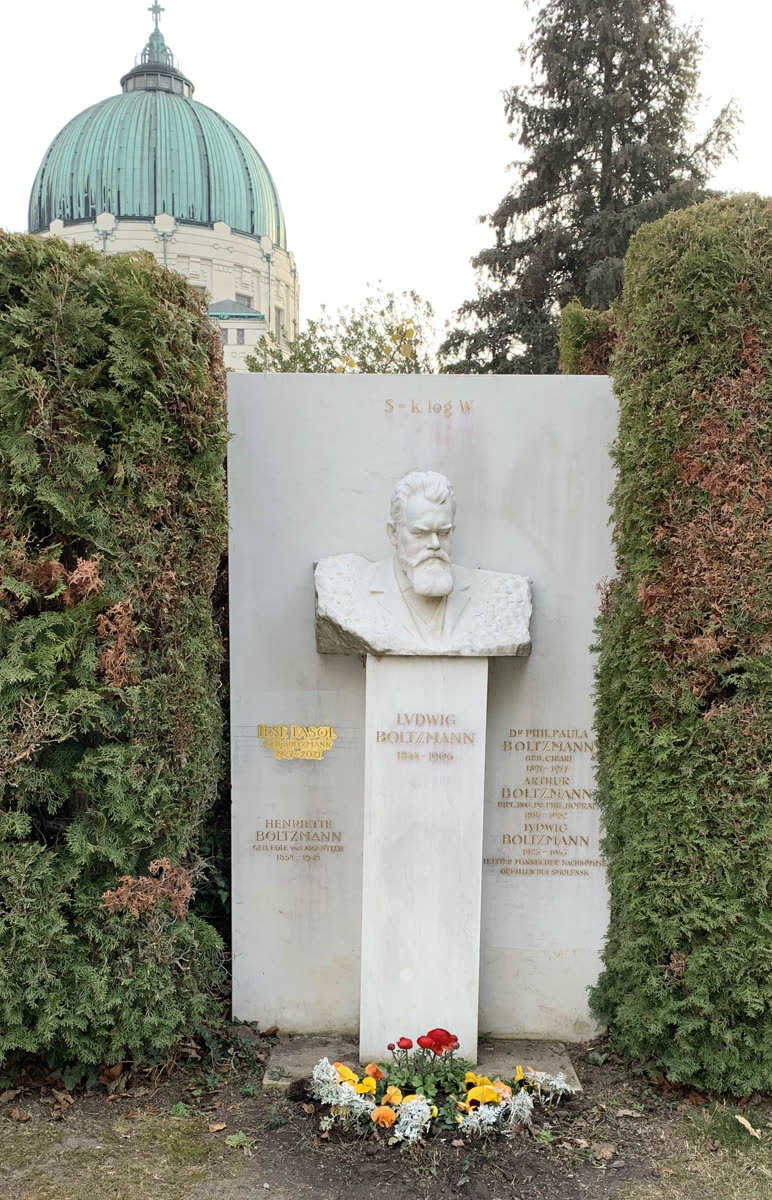
\includegraphics[width=\linewidth]{images/book4/boltzmann-grave.jpg}\par
{\footnotesize قبر بولتزمان.}
\end{minipage}
\end{history}

\section{تمارين}

\begin{exercise}[$\star$]\label{exo:b3:partition-functions:1}
تتقاسم أربعة هزازات أربعة كمّات. اكتب التوزيعات، وأعطِ وزن
كل منها، وتحقق من أن مجموعها يساوي عدد طرائق وضع أربعة
كمّات \omterm{def:b3:many-electron-atoms:indistinguishable}{غير قابلة للتمييز} في أربعة هزازات، $\binom{7}{3}$. أي التوزيعات هي
الأكثر احتمالًا؟
\end{exercise}

\begin{exercise}[$\star$]\label{exo:b3:partition-functions:2}
مستويان غير منحلين يفصل بينهما \qty{2.5}{kJ/mol}. احسب نسبة
إشغاليهما عند \qty{298.15}{K} وعند \qty{1000}{K}. وما النهاية في درجة حرارة
مرتفعة جدًا؟
\end{exercise}

\begin{exercise}[$\star$]\label{exo:b3:partition-functions:3}
% ledger: aw:Ar
احسب \omterm{def:b3:partition-functions:thermal-wavelength}{طول الموجة الحراري} لذرة أرغون عند \qty{298.15}{K} ودالة
تجزئتها الانسحابية في حجم \qty{1}{dm^3}.
\end{exercise}

\begin{exercise}[$\star$]\label{exo:b3:partition-functions:4}
% ledger: diat:N2.Be, diat:N2.ae, diat:HCl.Be, diat:HCl.ae
بأخذ $B_0 = \qty{1.990}{cm^{-1}}$ (\ce{N2}) و\qty{10.440}{cm^{-1}} (\ce{H^{35}Cl})، احسب $\theta_{\mathrm R}$ 
ودالة التجزئة الدورانية في درجات الحرارة المرتفعة لكل جزيء عند
\qty{298.15}{K}.
\end{exercise}

\begin{exercise}[$\star\star$]\label{exo:b3:partition-functions:5}
% ledger: diat:I2.we, diat:I2.wexe, diat:N2.we, diat:N2.wexe
العددان الموجيان للانتقالين الأساسيين للجزيئين \ce{I2} و\ce{N2} هما \qty{213.27}{cm^{-1}} 
و\qty{2329.92}{cm^{-1}}. احسب $\theta_{\mathrm V}$، و$q^{\mathrm V}$ عند \qty{298.15}{K}، ونسبة الجزيئات
التي ليست في $v = 0$.
\end{exercise}

\begin{exercise}[$\star\star$]\label{exo:b3:partition-functions:6}
% ledger: diat:NO.split, lev:Cl.2P1_2
احسب دالة التجزئة الإلكترونية عند \qty{298.15}{K} للجزيء \ce{NO} (مستويان منحلان
مرتين يفصل بينهما \qty{119.73}{cm^{-1}}) ولذرة الكلور (المستوى الأساسي ${}^2P_{3/2}$
والمستوى ${}^2P_{1/2}$ عند \qty{882.35}{cm^{-1}}). ما نسبة جزيئات \ce{NO} في
المستوى الأعلى؟ وإلامَ تؤول $q^{\mathrm E}(\ce{NO})$ في درجة حرارة مرتفعة؟
\end{exercise}

\begin{exercise}[$\star\star$]\label{exo:b3:partition-functions:7}
انطلاقًا من $q^{\mathrm T} = V/\Lambda^3$، استنتج الطاقة الداخلية والسعة الحرارية عند
حجم ثابت لمول واحد من غاز مثالي أحادي الذرة، واحسب $U - U(0)$ عند
\qty{298.15}{K}.
\end{exercise}

\begin{exercise}[$\star\star$]\label{exo:b3:partition-functions:8}
% ledger: aw:Ar, s0:Ar_g
استعمل معادلة زاكور--تيترود لحساب الإنتروبيا المولية القياسية
للأرغون عند \qty{298.15}{K}؛ وقارن بالقيمة الجدولية
\qty{154.846}{J.K^{-1}.mol^{-1}}. وكم تتغير إذا قُسم الضغط على 10؟
\end{exercise}

\begin{exercise}[$\star\star$]\label{exo:b3:partition-functions:9}
% ledger: diat:HCl.Be, diat:HCl.ae
احسب المساهمة الدورانية في الإنتروبيا المولية القياسية للجزيء
\ce{H^{35}Cl} عند \qty{298.15}{K} ($\theta_{\mathrm R} = \qty{15.02}{K}$).
\end{exercise}

\begin{exercise}[$\star\star\star$]\label{exo:b3:partition-functions:10}
بمعاملة $J$ متغيرًا متصلًا، بيّن أن المستوى الدوراني الأكثر إشغالًا في
جزيء خطي يقع قرب $J_{\max} = \sqrt{T/2\theta_{\mathrm R}} - \frac12$. واحسبه للجزيء \ce{HCl}
($\theta_{\mathrm R} = \qty{15.02}{K}$) وللجزيء \ce{CO} ($\theta_{\mathrm R} = \qty{2.766}{K}$) عند \qty{300}{K}. لماذا يكون
فرعا الحزمة تحت الحمراء في أشدهما على بعد بضعة خطوط من المركز؟
\end{exercise}

\begin{exercise}[$\star\star\star$]\label{exo:b3:partition-functions:11}
% ledger: diat:H2.Be, diat:H2.ae
تعطي علاقة أويلر--ماكلورين $\sum_{J\ge0}f(J) \approx \int_0^\infty f(J)\dd J + \frac12f(0) -
\frac1{12}f'(0)$. طبّقها على $f(J) = (2J+1)\eu^{-\theta J(J+1)/T}$ وبيّن أن $q^{\mathrm R} \approx T/\theta +
\frac13$. ومن أجل أي درجات حرارة تكون $T/\theta$ صحيحة في حدود 1\,\%؟ وهل هي مقبولة للجزيء \ce{H2}
($B_0 = \qty{59.32}{cm^{-1}}$) عند \qty{298.15}{K}؟
\end{exercise}

\begin{exercise}[$\star\star\star$]\label{exo:b3:partition-functions:12}
% ledger: diat:I2.we, diat:I2.wexe
بيّن أن الإنتروبيا المولية الاهتزازية تؤول إلى الصفر حين $T \ll \theta_{\mathrm V}$ وإلى
$R[1 + \ln(T/\theta_{\mathrm V})]$ حين $T \gg \theta_{\mathrm V}$. واحسب العبارة الدقيقة وهذه
النهاية للجزيء \ce{I2} ($\theta_{\mathrm V} = \qty{306.9}{K}$) عند \qty{298.15}{K}، وعلّق.
\end{exercise}

\section{مسألة: عدّ إنتروبيا النيتروجين}

\begin{problem}[{مسألة نهاية الأسبوع --- عدّ إنتروبيا النيتروجين: المساهمات
الانسحابية والدورانية والاهتزازية والإلكترونية في
إنتروبياه القياسية، محسوبةً من طيفه ومقارنةً بالجدول}]
\label{pb:b3:partition-functions:1}
% ledger: aw:N, diat:N2.Be, diat:N2.ae, diat:N2.we, diat:N2.wexe, s0:N2_g, const:h, const:kB, const:NA, const:c
النيتروجين الغاز الرئيسي في الهواء. وتُحسب هنا إنتروبياه المولية القياسية عند
\qty{298.15}{K} من كتلته المولية، \qty{28.014}{g/mol}، ومن
ثوابته الطيفية: $B_e = \qty{1.998241}{cm^{-1}}$، $\alpha_e = \qty{0.017318}{cm^{-1}}$، $\omega_e =
\qty{2358.57}{cm^{-1}}$، $\omega_ex_e = \qty{14.324}{cm^{-1}}$؛ وحده الإلكتروني الأساسي ${}^1\Sigma_g^+$.
الضغط القياسي $p^\circ = \qty{1}{bar}$؛ $k = \qty{1.380649e-23}{J/K}$، $h = \qty{6.62607015e-34}{J.s}$.

\medskip\noindent\textbf{الجزء الأول --- الانسحاب.}
\begin{enumerate}
  \item احسب كتلة جزيء واحد.
  \item احسب طول موجته الحراري عند \qty{298.15}{K}.
  \item احسب الحجم المتاح لكل جزيء، $kT/p^\circ$.
  \item استنتج $q^{\mathrm T}/N$، وعلّق على قيمته.
  \item احسب الإنتروبيا المولية الانسحابية.
  \item وكم تتغير عند نصف الضغط؟
\end{enumerate}

\medskip\noindent\textbf{الجزء الثاني --- الدوران.}
\begin{enumerate}[resume]
  \item احسب $B_0$.
  \item احسب $\theta_{\mathrm R}$.
  \item أعطِ \omterm{def:b3:partition-functions:symmetry-number}{عدد التناظر} وبيّن ما الذي يأخذه في الحسبان.
  \item احسب $q^{\mathrm R}$ عند \qty{298.15}{K}.
  \item هل صيغة درجات الحرارة المرتفعة مسوَّغة؟
  \item احسب الإنتروبيا المولية الدورانية.
  \item بإهمال أوزان سبين النوى، أي المستويات الدورانية هو الأكثر
        إشغالًا؟
\end{enumerate}

\medskip\noindent\textbf{الجزء الثالث --- الاهتزاز والحالات الإلكترونية.}
\begin{enumerate}[resume]
  \item احسب الكمّ الاهتزازي $G(1) - G(0)$.
  \item احسب $\theta_{\mathrm V}$.
  \item احسب $q^{\mathrm V}$ عند \qty{298.15}{K}.
  \item ما نسبة الجزيئات في $v = 1$؟
  \item احسب الإنتروبيا المولية الاهتزازية.
  \item ما المساهمة الإلكترونية؟ ولماذا يمكن إهمال الحالات الإلكترونية
        المثارة؟
\end{enumerate}

\medskip\noindent\textbf{الجزء الرابع --- المجموع والمقارنة.}
\begin{enumerate}[resume]
  \item اجمع المساهمات.
  \item قارن بالقيمة الجدولية \qty{191.609}{J.K^{-1}.mol^{-1}}.
  \item على أي قياسات تقوم القيمة المسعرية في الجدول؟
  \item لماذا يمكن للجداول أن تترك سبين النوى جانبًا؟
  \item اذكر النتيجة: الإنتروبيا المولية القياسية للنيتروجين عند \qty{298.15}{K}
        محسوبةً من ثوابته الطيفية.
\end{enumerate}
\end{problem}
